\chapter{Workflow (to be) na notação BPMN}\label{sec:workflow-to-be}

Enquanto o workflow AS-IS registra a situação encontrada, o workflow TO-BE representa o processo depois da introdução do sistema, servindo de referência para o que foi implementado. A Figura~\ref{fig:workflow-to-be} apresenta o fluxo proposto.

\begin{figure}[H]
    \caption{Workflow TO-BE}
    \label{fig:workflow-to-be}
    \centering
    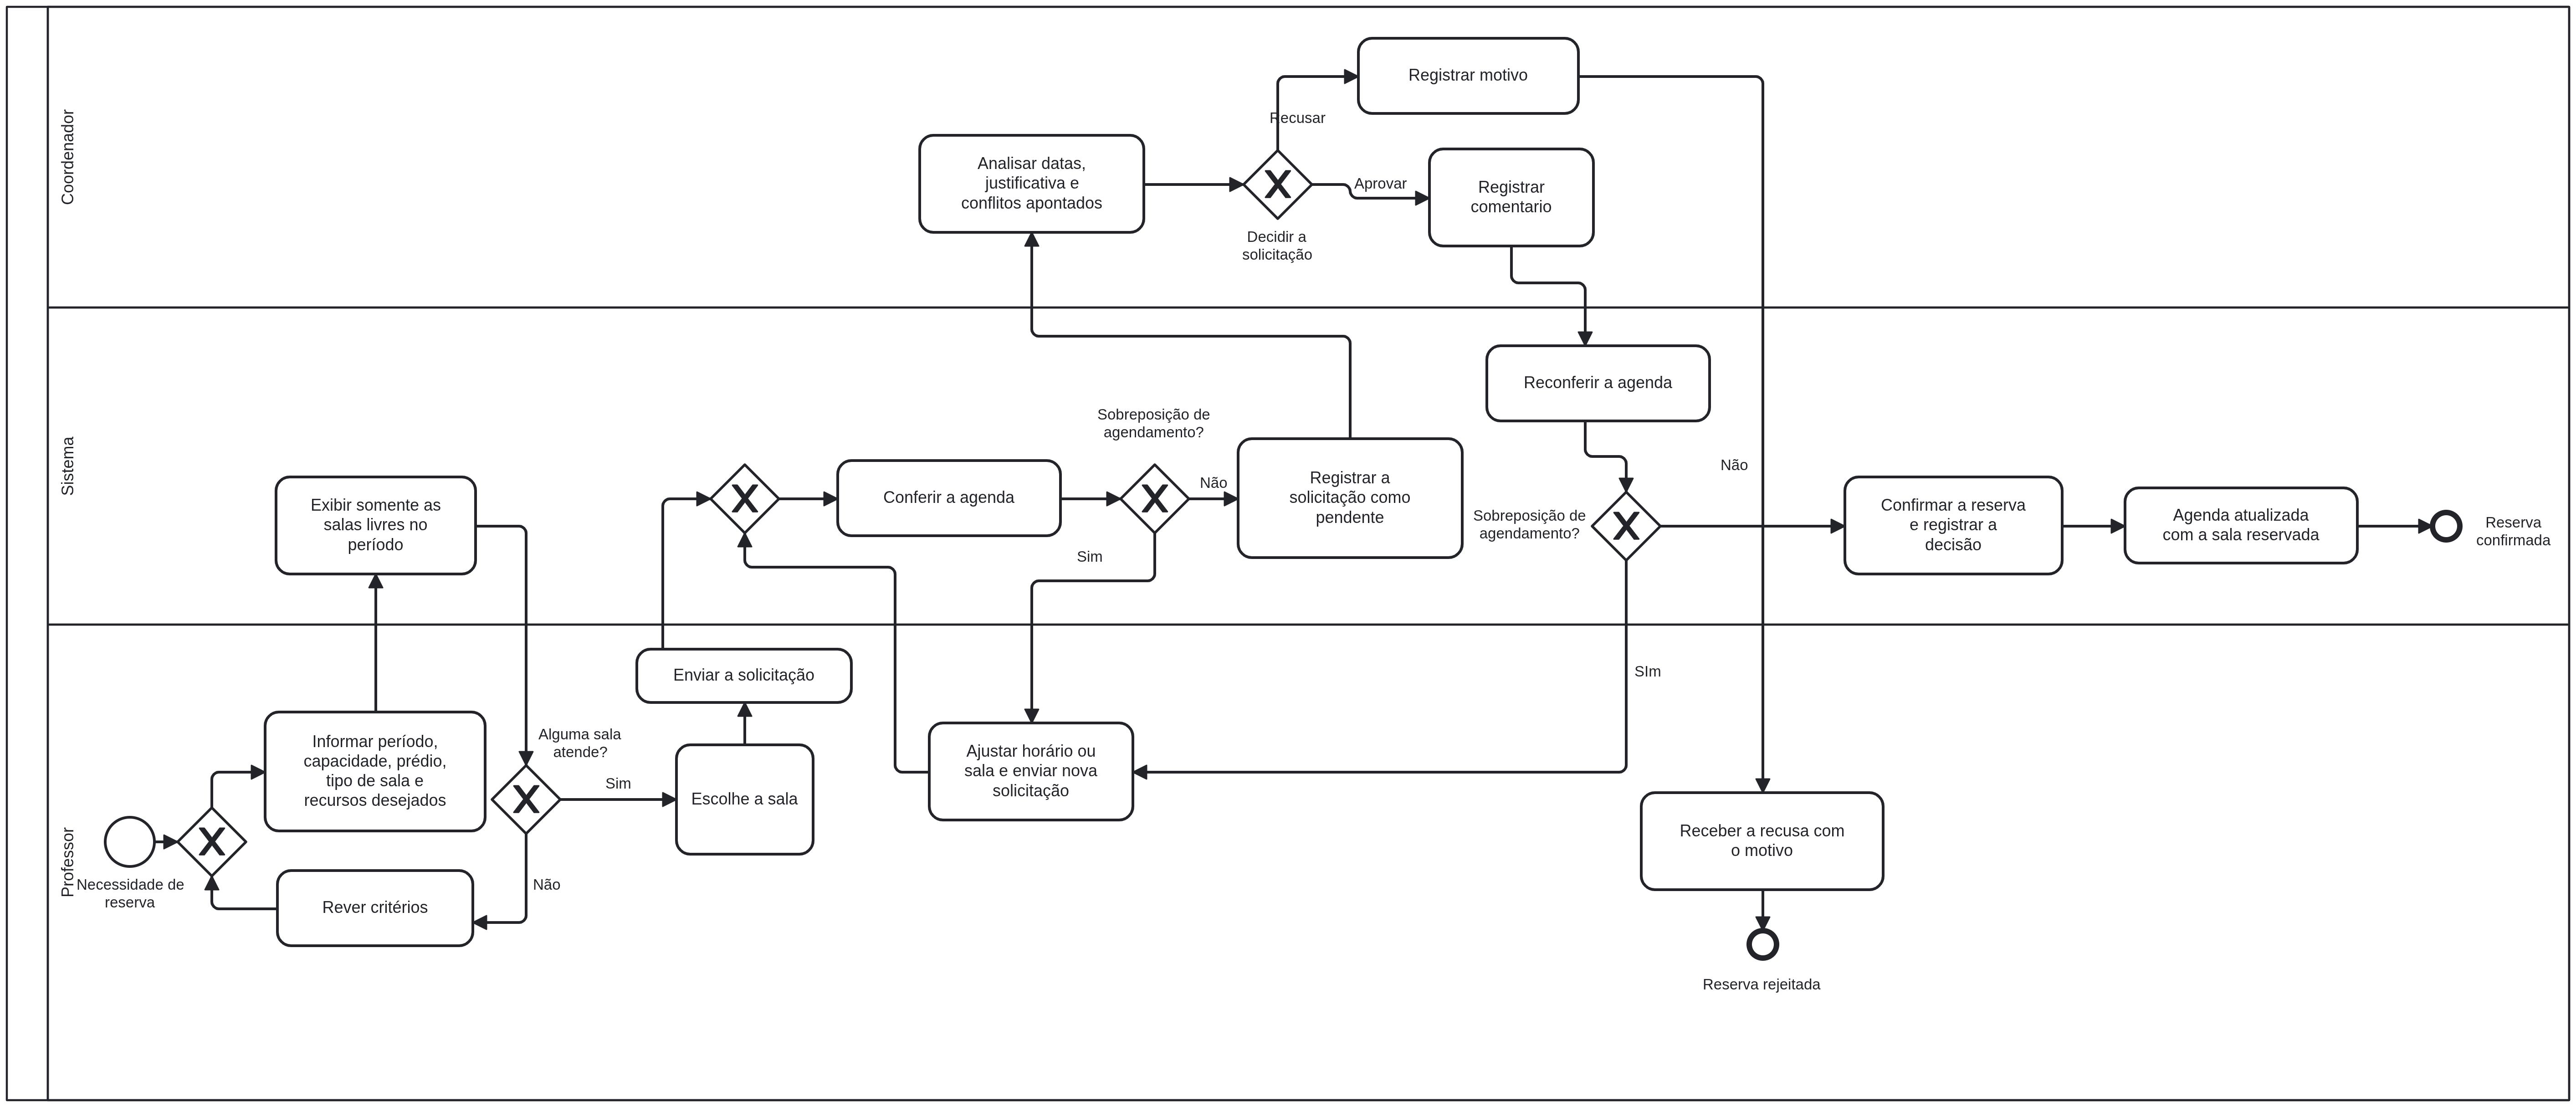
\includegraphics[width=\textwidth]{imagens/workflow-to-be.png}

    {\footnotesize \textbf{Fonte:} O autor.}
\end{figure}